\documentclass{../source/Experiment}

\major{信息工程}
\name{}
\title{FIR数字滤波器设计与使用}
\stuid{}
\college{信息与电子工程学院}
\date{\today}
\lab{——}
\course{数字信号处理}
\instructor{徐元欣}
\grades{}
\expname{FIR数字滤波器设计与使用}
\exptype{设计}
\partner{——}
\begin{document}
\makeheader
\section{实验目的和要求}
设计和应用FIR低通滤波器。掌握FIR数字滤波器的窗函数设计法,了解设计参数(窗型、窗长)的影响。
\section{实验内容和步骤}
编写MATLAB程序,完成以下工作。

2-1 设计两个FIR低通滤波器,截止频率$ \rm \omega C = 0.5 \pi$。

(1)用矩形窗,窗长N=31。得出第一个滤波器的单位抽样响应序列$ \rm h_1(1)$。记下$ \rm h_1(1)$的各个抽样值,显示$ \rm h_1(1)$的图形(用stem(.))。求出该滤波器的频率响应(的N个抽样)$ \rm H_1(k)$,显示$| \rm H_1(k)|$的图形(用plot(.))。

(2)用汉明窗,窗长N=31。得出第二个滤波器的单位抽样响应序列h2(n)。记下h2(n)的各个抽样值,显示h2(n)的图形。求出滤波器的频率响应H2(k),显示|H2(k)|的图形。

(3)由图形,比较$ \rm h_1(1)$与$ \rm h_2(n)$的差异,$| \rm H_1(k)|$与$\rm |H_2(k)|$的差异。

2-2 产生长度为200点、均值为零的随机信号序列x(n)(用rand(1,200)  0.5)。显示x(n)。求出并显示其幅度谱|X(k)|,观察特征。

2-3 滤波

(1)将x(n)作为输入,经过第一个滤波器后的输出序列记为$ \rm y_1(n)$,其幅度谱记为$|\rm Y_1(k)|$。显示|X(k)|与$\rm |Y_1(k)|$,讨论滤波前后信号的频谱特征。

(2)将x(n)作为输入,经过第二个滤波器后的输出序列记为$\rm y_2(n)$,其幅度谱记为$|\rm Y_2(k)|$。比较$|\rm Y_1(k)|$与$|\rm Y_2(k)|$的图形,讨论不同的窗函数设计出的滤波器的滤波效果。

2-4 设计第三个FIR低通滤波器,截止频率$\rm \omega C=0.5\pi$。用矩形窗,窗长N=127。用它对x(n)进行滤波。显示输出信号$ \rm y_3(n)$的幅度谱$\rm |Y_3(k)|$,并与$\rm |Y_1(k)|$比较,讨论不同的窗长设计出的滤波器的滤波效果。
\section{主要仪器设备}
MATLAB编程。
\section{操作方法和实验步骤}
(参见“二、实验内容和步骤”)
\section{实验数据记录和处理}
\subsection{列出MATLAB程序清单,加注释。}

\lstinputlisting[
    language = matlab,
    title = {第四次实验代码}
]{src/exp4new.m}

\subsection{列出计算结果,包括$\rm h_1(n)$和$\rm h_2(n)$的各个抽样值,$\rm |H_1(k)|$、$\rm |H_2(k)|$、$\rm |X(k)|$、$\rm |Y_1(k)|$、$\rm |Y_2(k)|$和$\rm |Y_3(k)|$的图形。}

$\rm h_1(n)$和$\rm h_2(n)$
\begin{figure}[H]
    \centering
    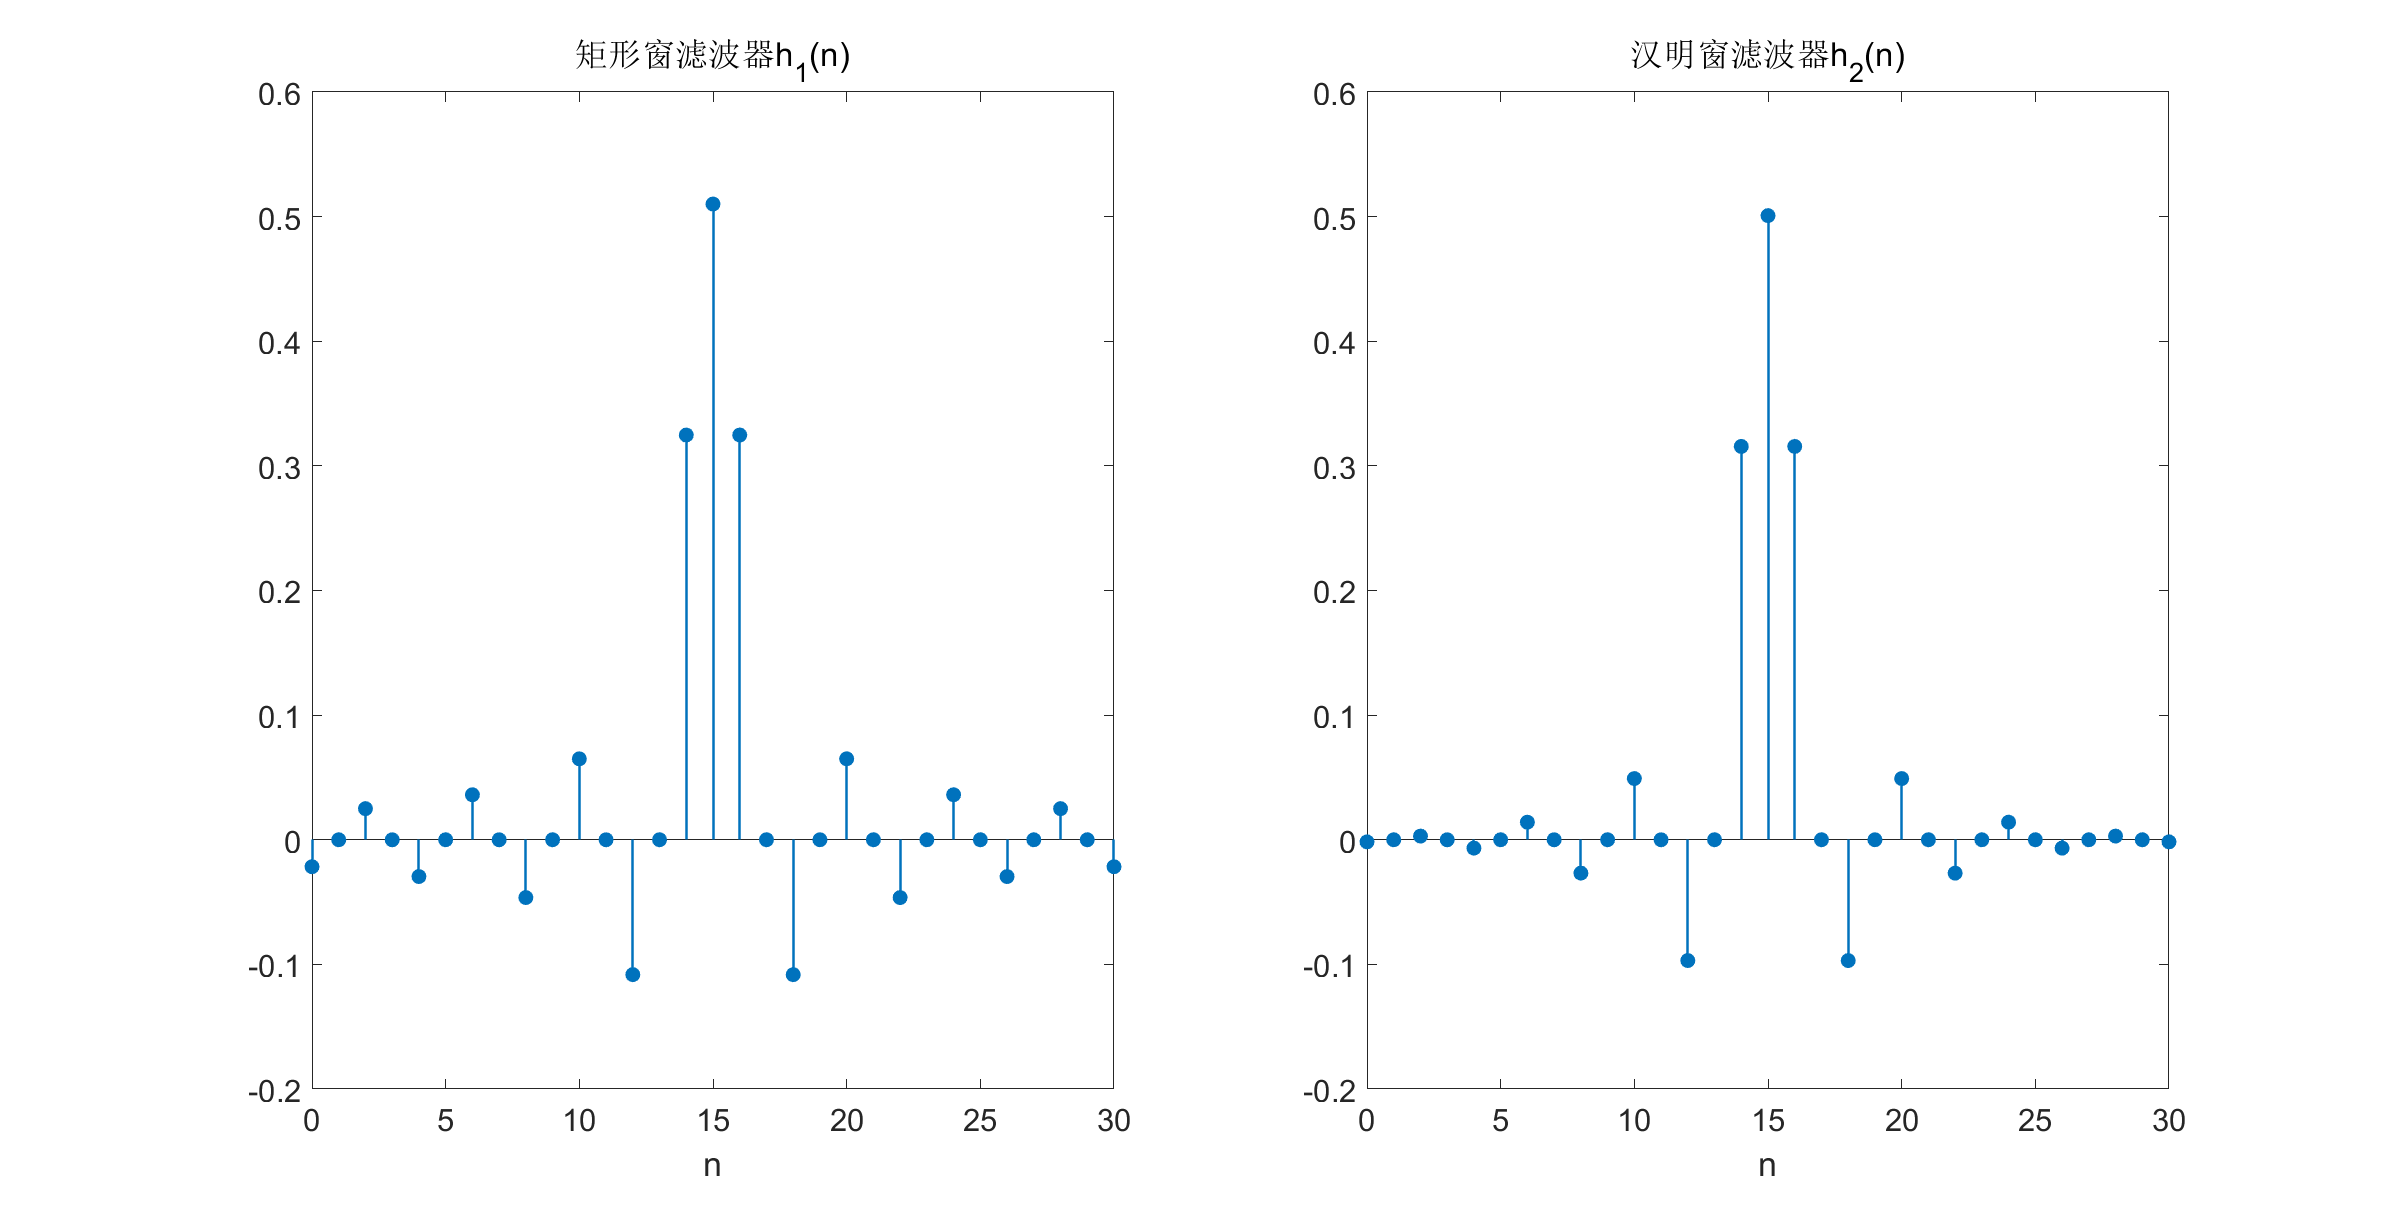
\includegraphics[width = 0.8\textwidth]{src/exp4-5-2-1.png}
\end{figure}

$\rm |H_1(k)|$、$\rm |H_2(k)|$、$\rm |X(k)|$
\begin{figure}[H]
    \centering
    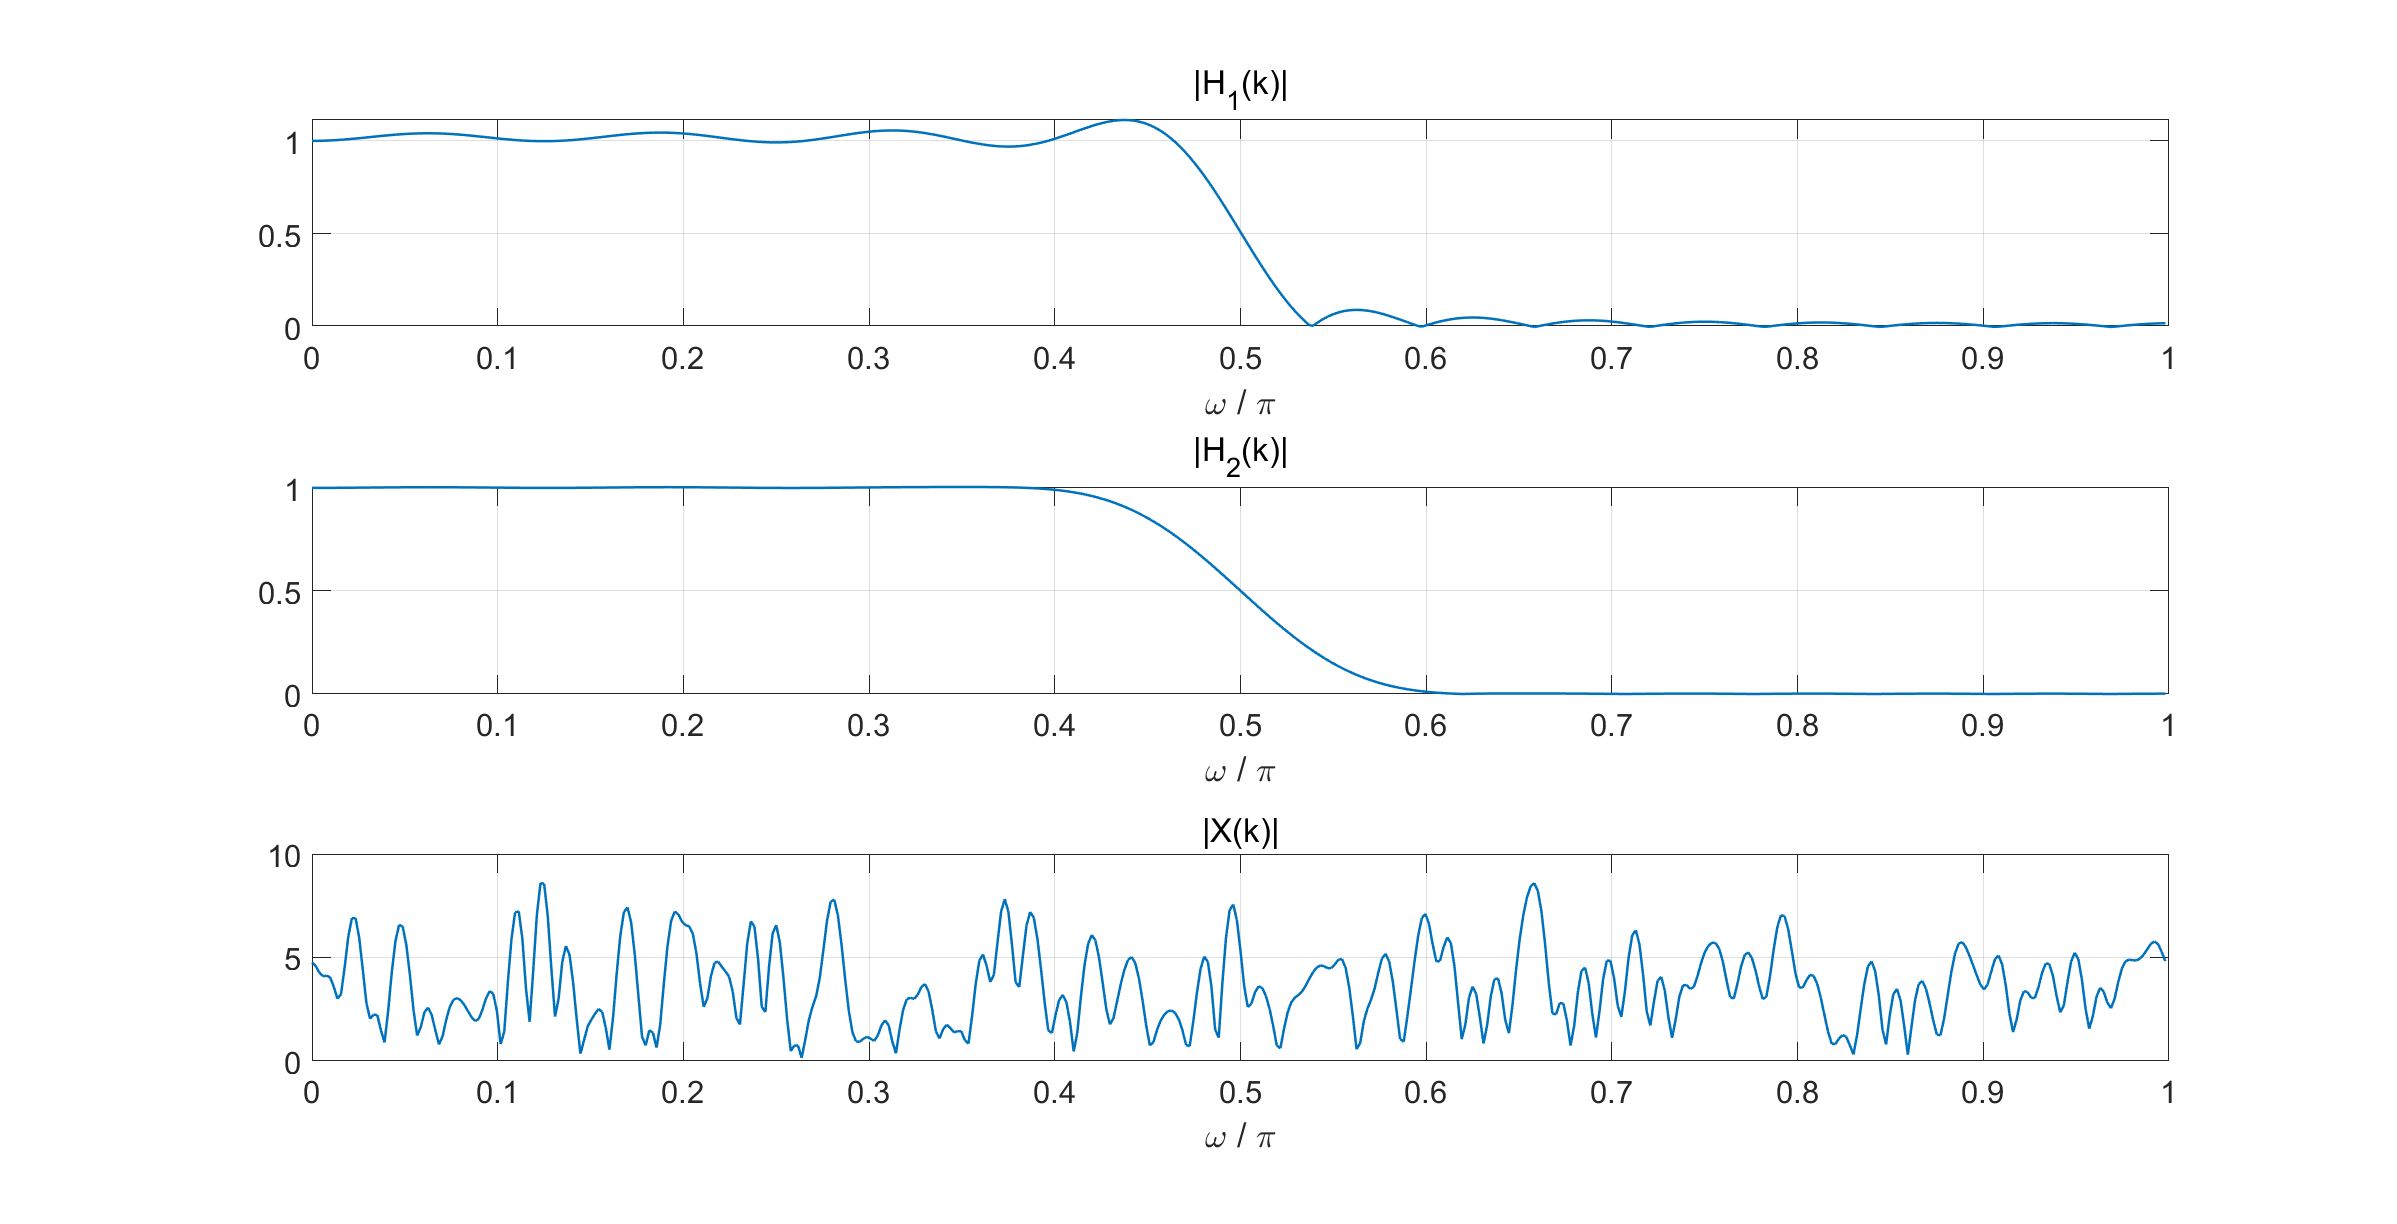
\includegraphics[width = 1\textwidth]{src/exp4-5-2-2.png}
\end{figure}

$\rm |Y_1(k)|$、$\rm |Y_2(k)|$和$\rm |Y_3(k)|$
\begin{figure}[H]
    \centering
    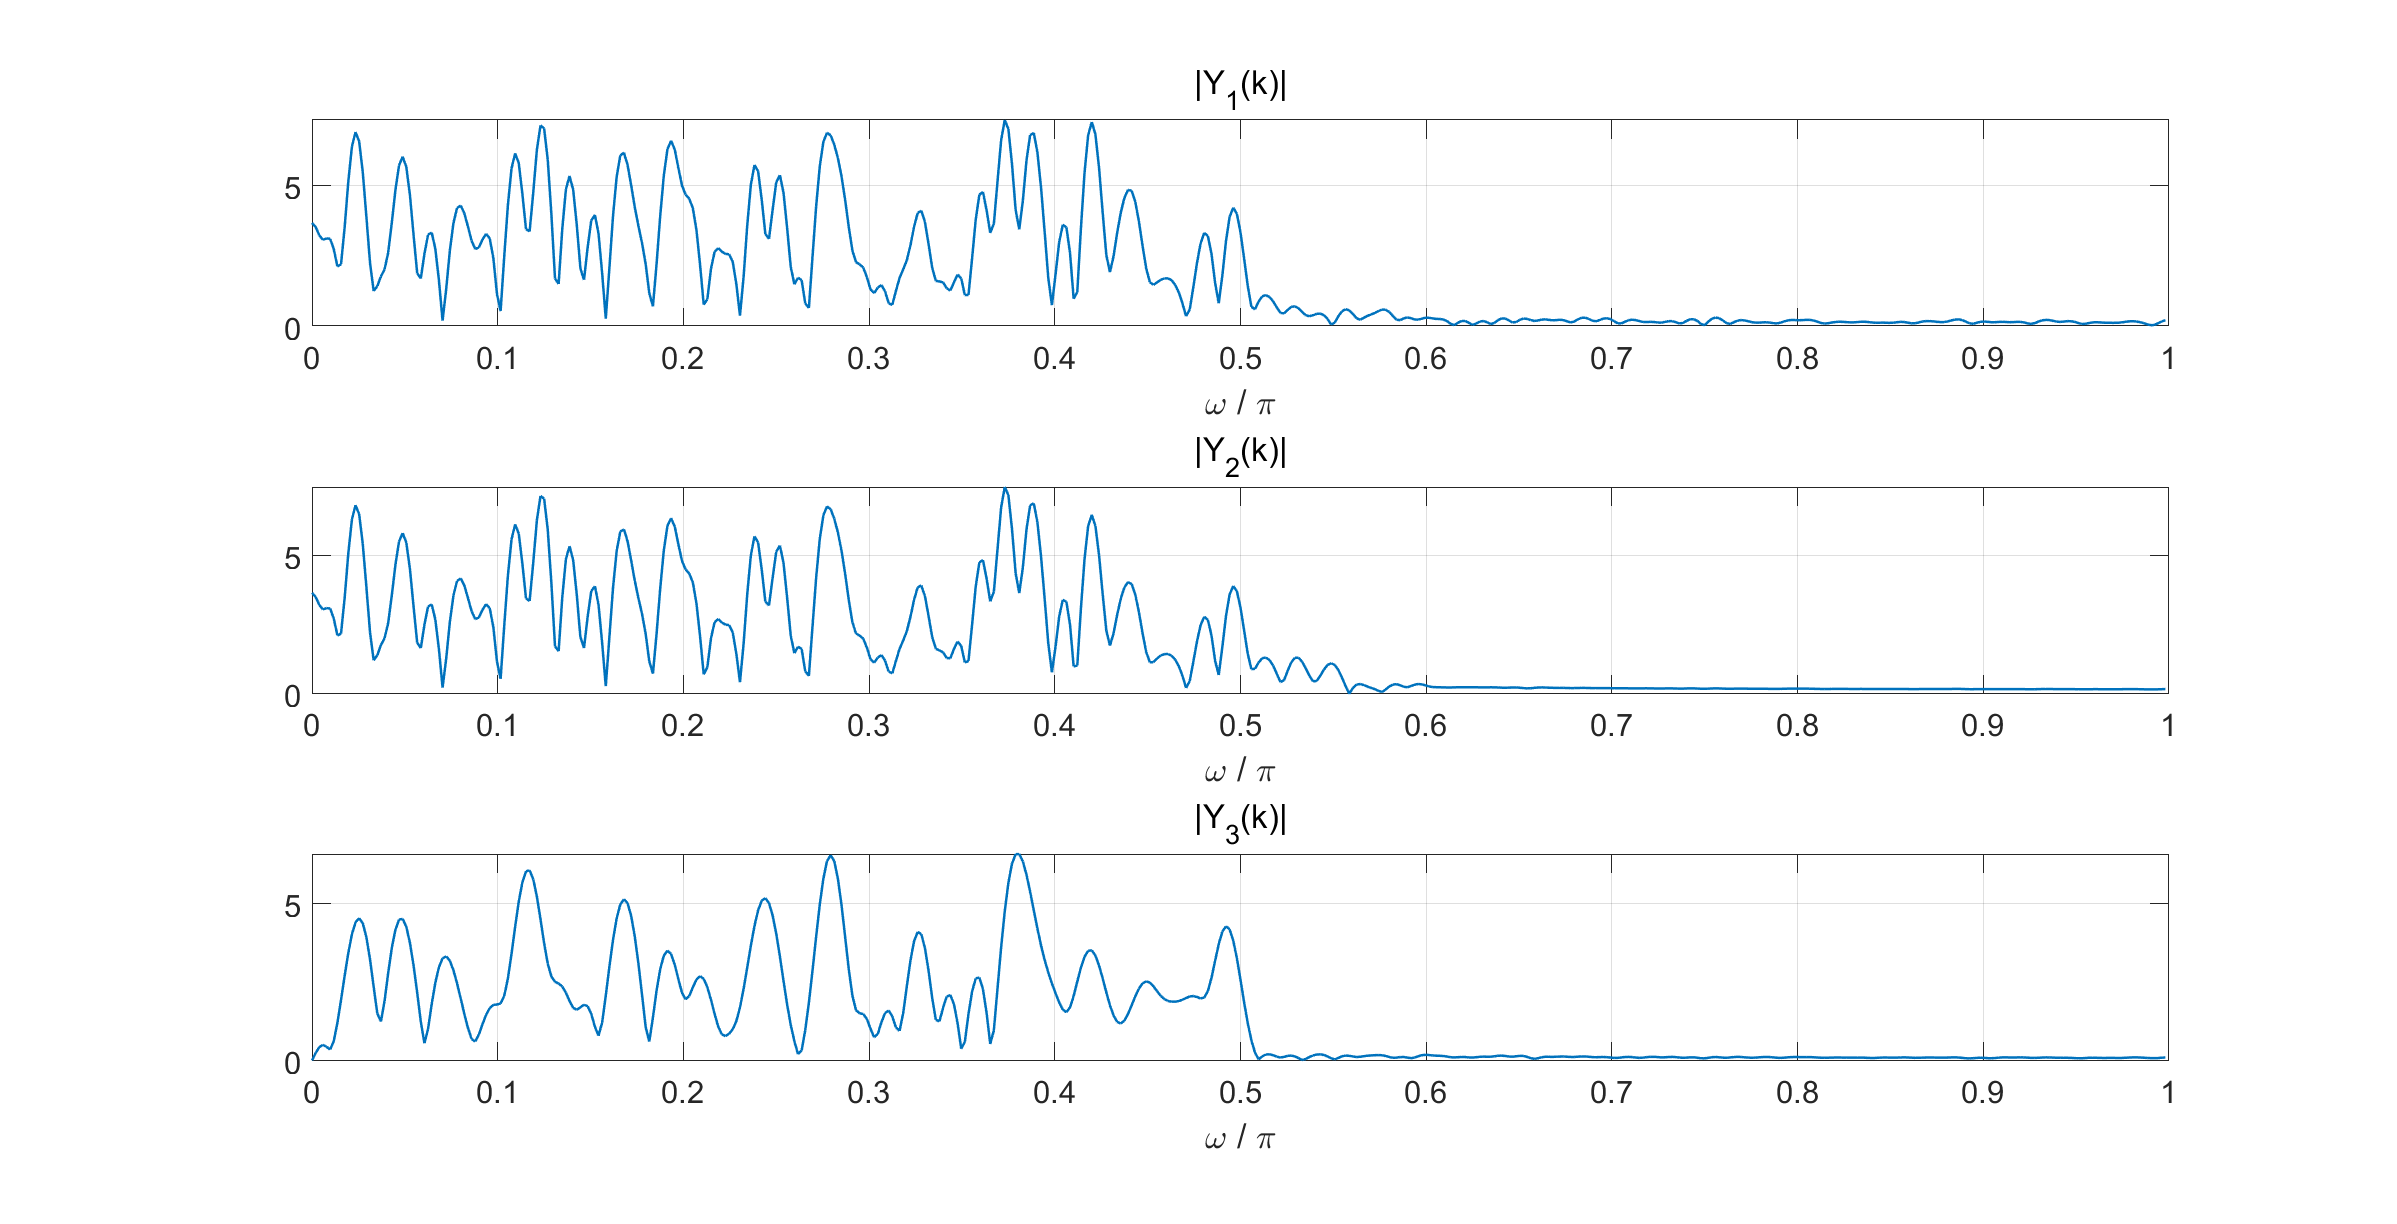
\includegraphics[width = 1\textwidth]{src/exp4-5-2-3.png}
\end{figure}
\section{实验结果与分析}
\subsection{2-1}
\begin{figure}[H]
    \centering
    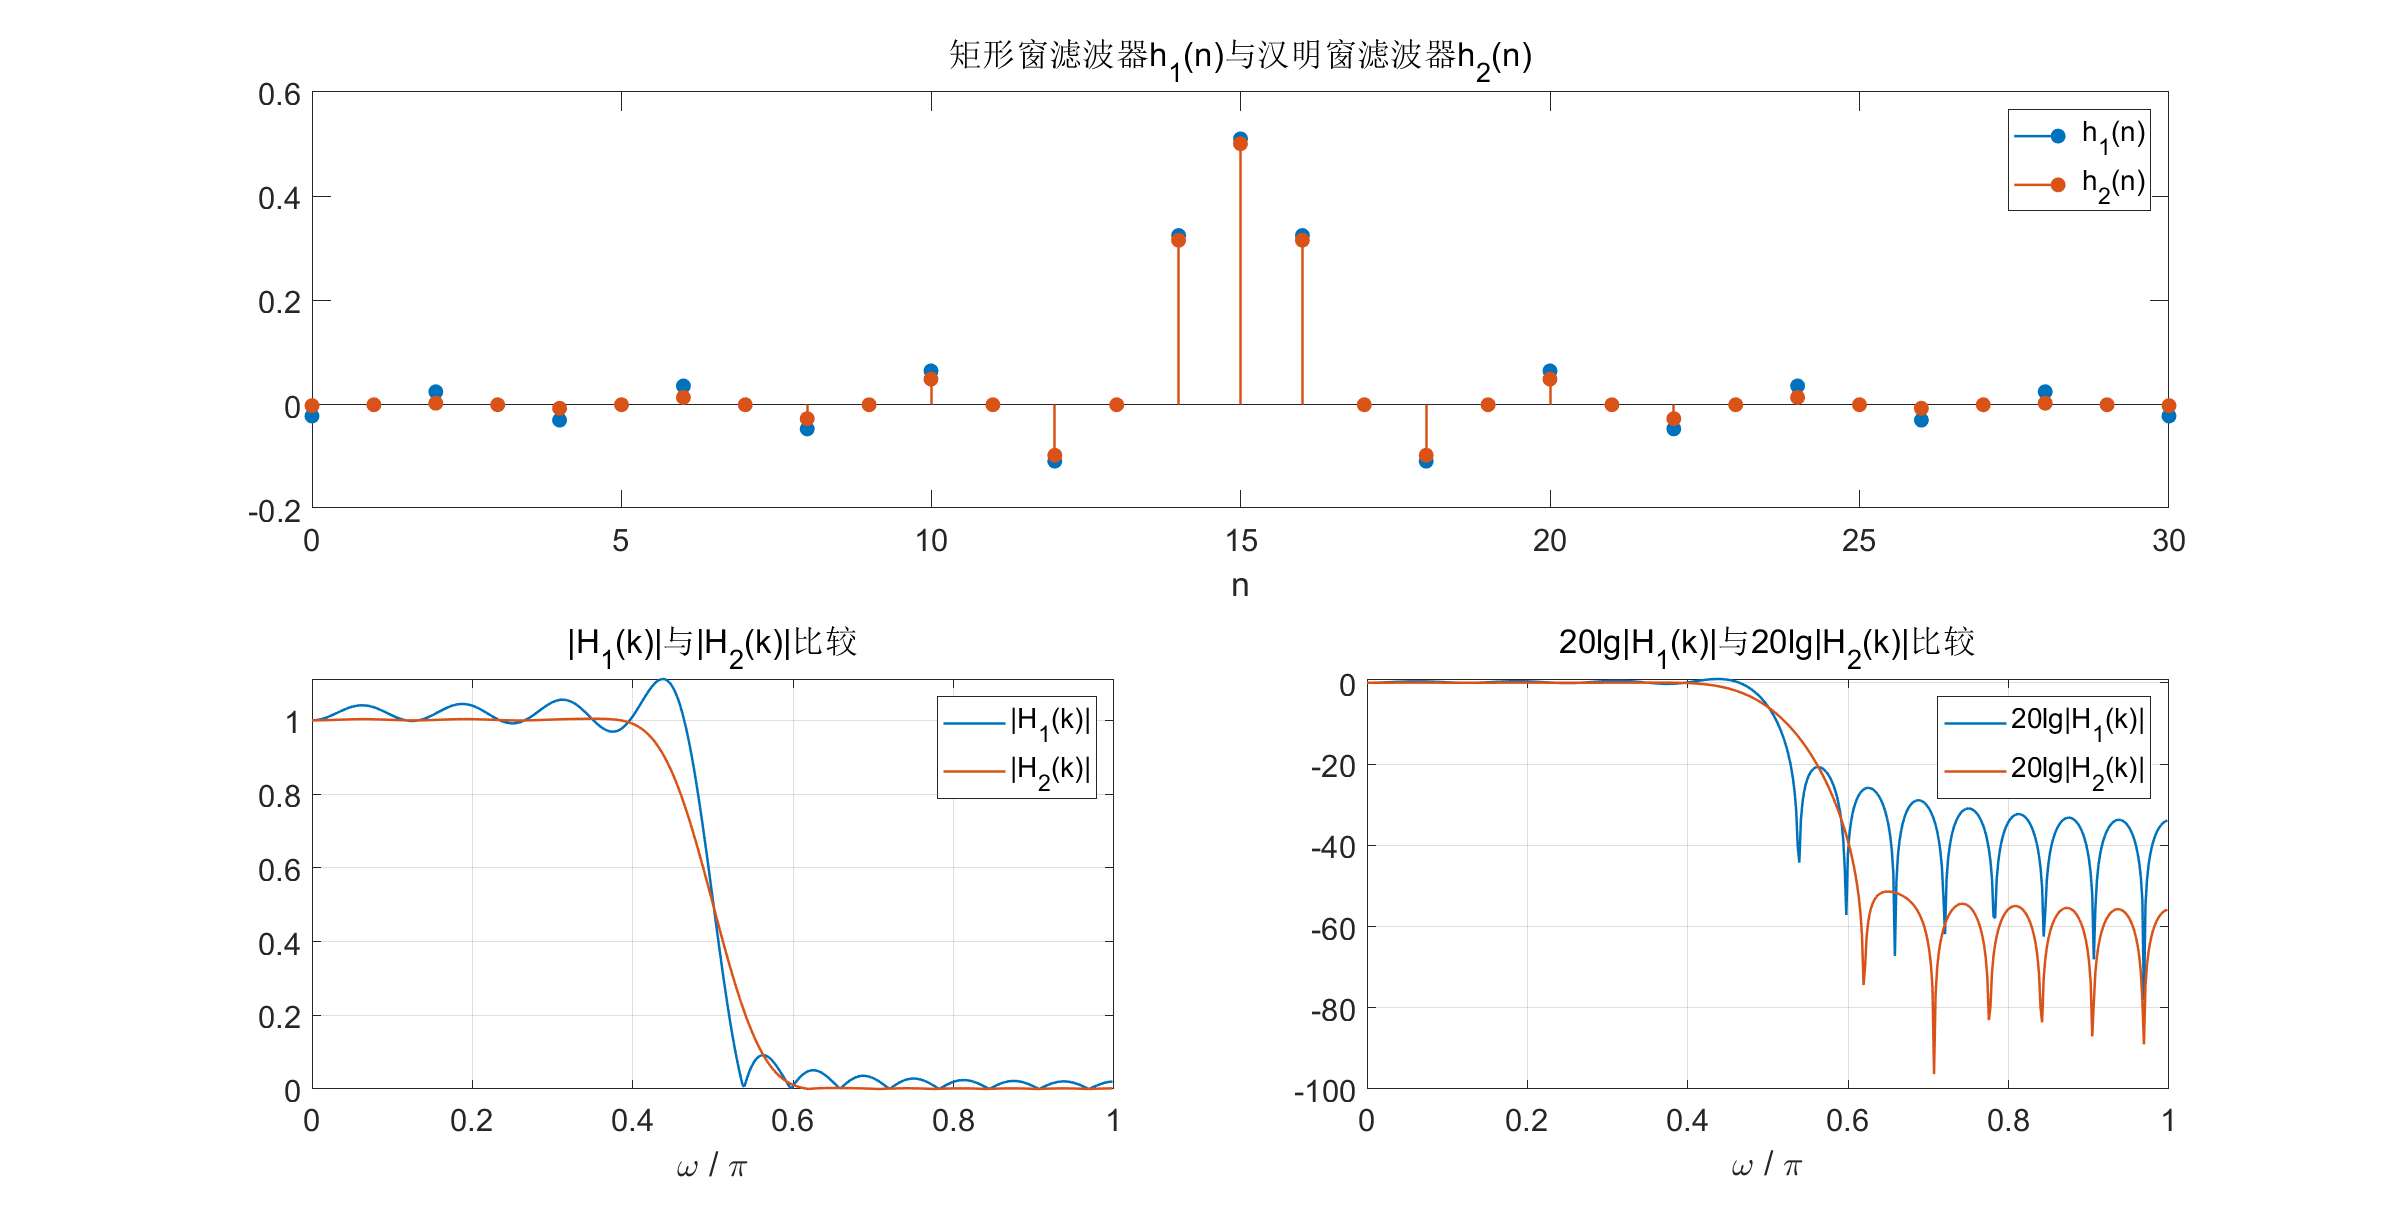
\includegraphics[width = 1\textwidth]{src/exp4-2-1.png}
\end{figure}
观察$\rm h_1(n)$和$\rm h_2(n)$可知,两个序列的主瓣上的取样点数相同,值几乎相等,最大值都相同,但是旁瓣上$\rm h_1(n)$在靠近0和30处的波动较大。
观察$\rm |H_1(k)|$和$\rm |H_2(k)|$可知,通带内,$\rm |H_1(k)|$的波动较大,但过渡带宽度小;$\rm |H_2(k)|$波动很小,过渡带宽度大。
而而$\rm |H_1(k)|$的最小衰减为-20dB左右,$\rm |H_2(k)|$的最小衰减为-53dB左右,$\rm |H_2(k)|$的最小衰减更小。

\subsection{2-2}
\begin{figure}[H]
    \centering
    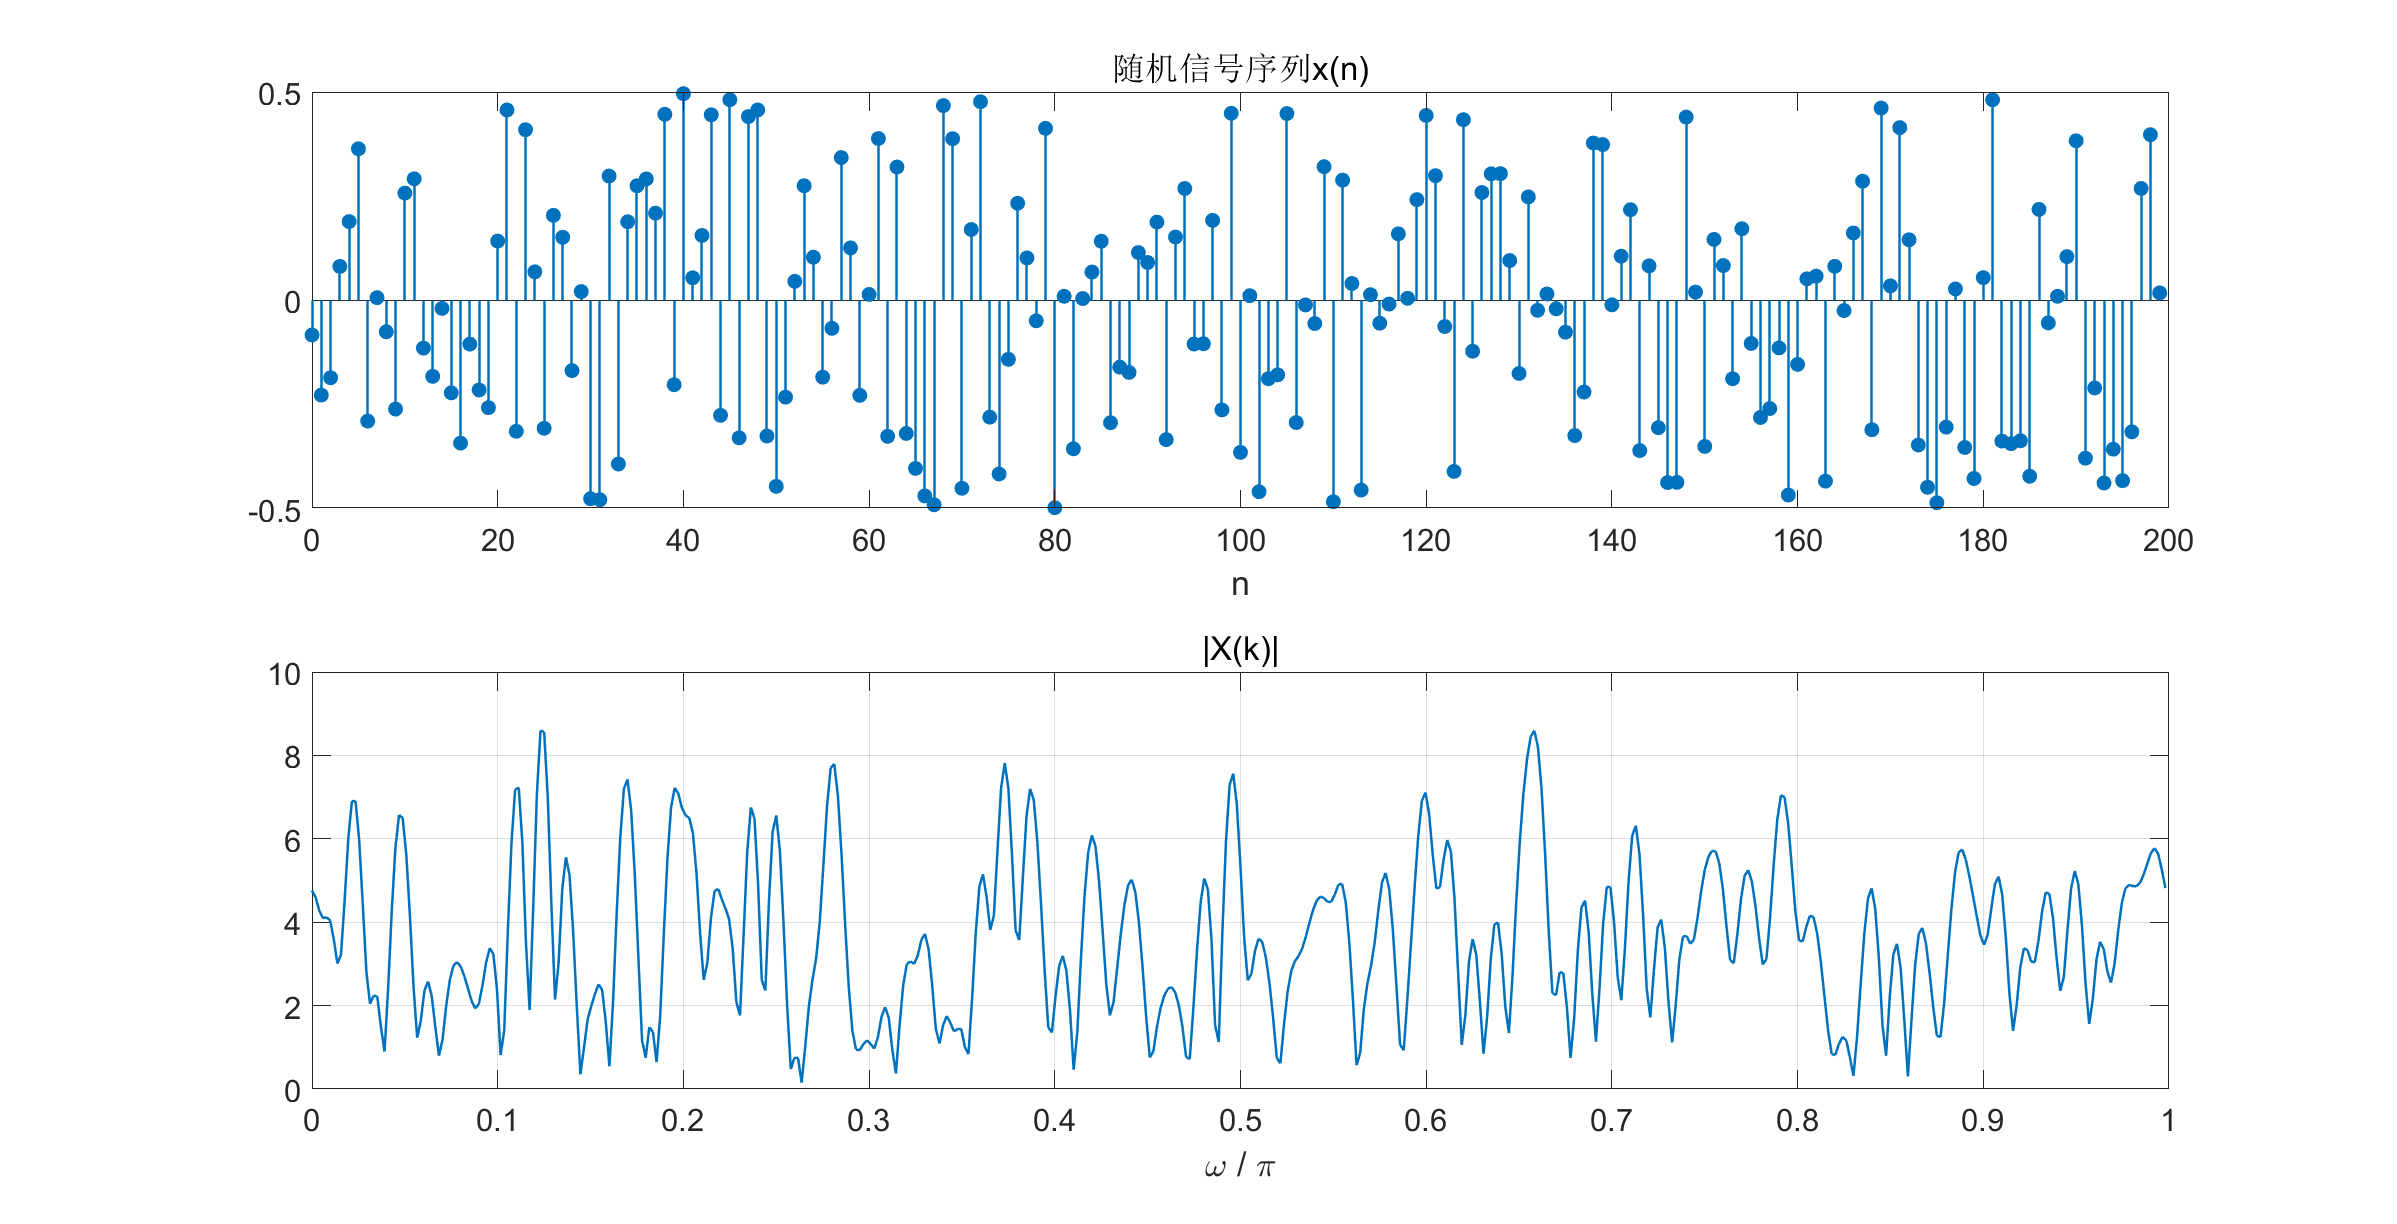
\includegraphics[width = 1\textwidth]{src/exp4-2-2.png}
\end{figure}
从图中可以看出,输入的是随机序列,其低频和高频分量都存在,利于我们之后的分析。
\subsection{2-3}
比较|X(k)|与滤波后的$\rm |Y_1(k)|$。
\begin{figure}[H]
    \centering
    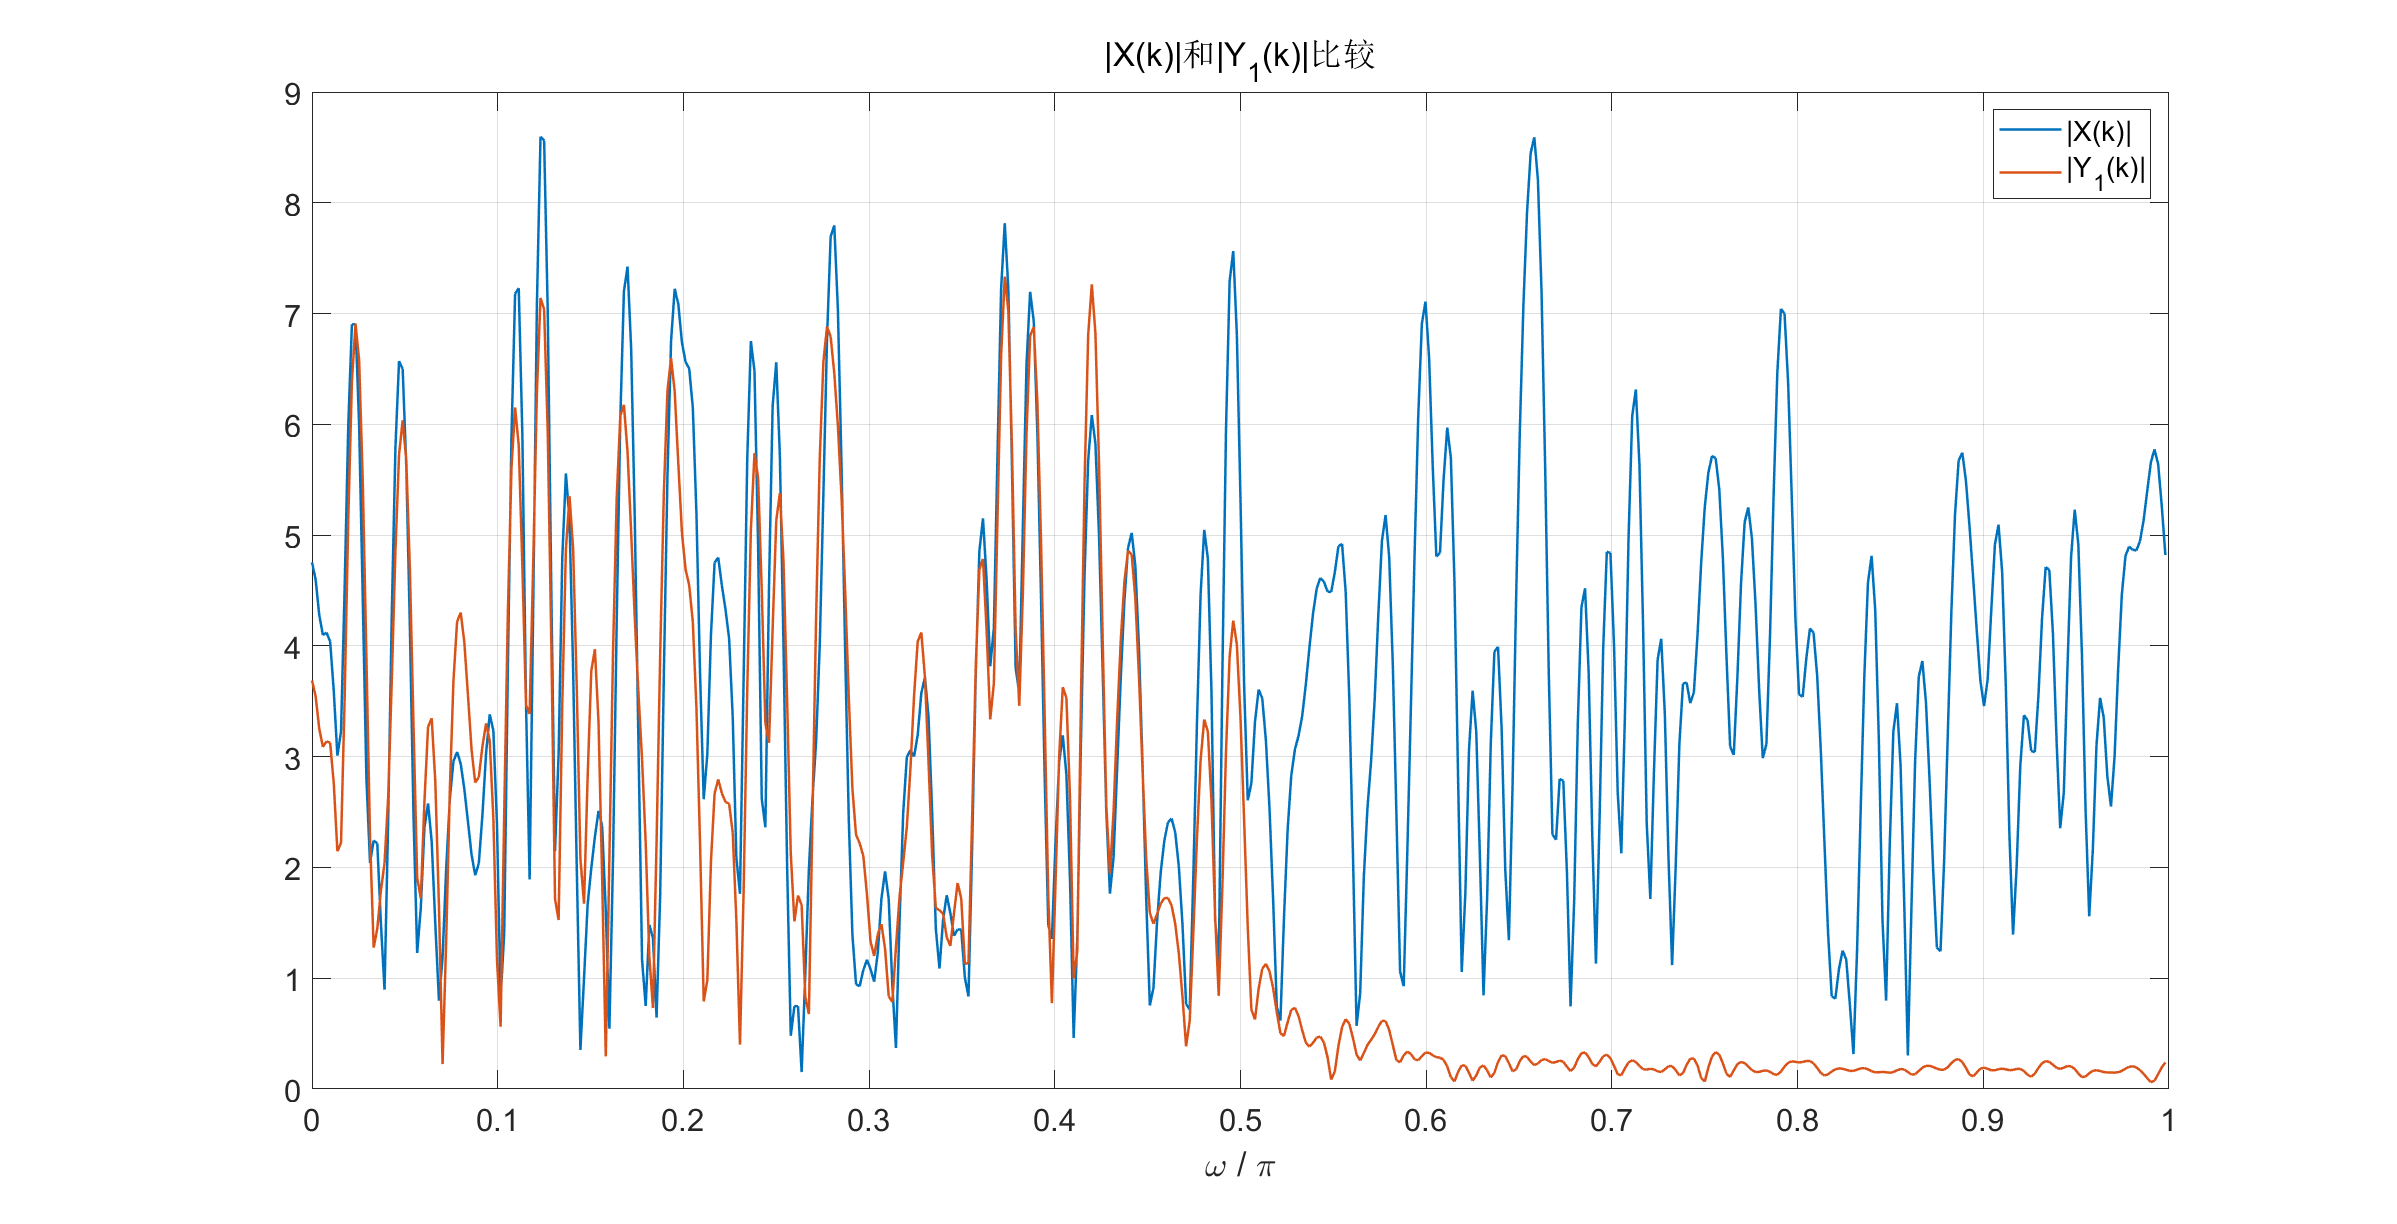
\includegraphics[width = 1\textwidth]{src/exp4-2-3-1.png}
\end{figure}
从图中可以看出,经过滤波后,大于截至频率$\rm \omega _c = 0.5 \pi$的高频分量几乎为0,而低频分量基本保留。

比较不同的窗函数设计出的滤波器的滤波效果。
\begin{figure}[H]
    \centering
    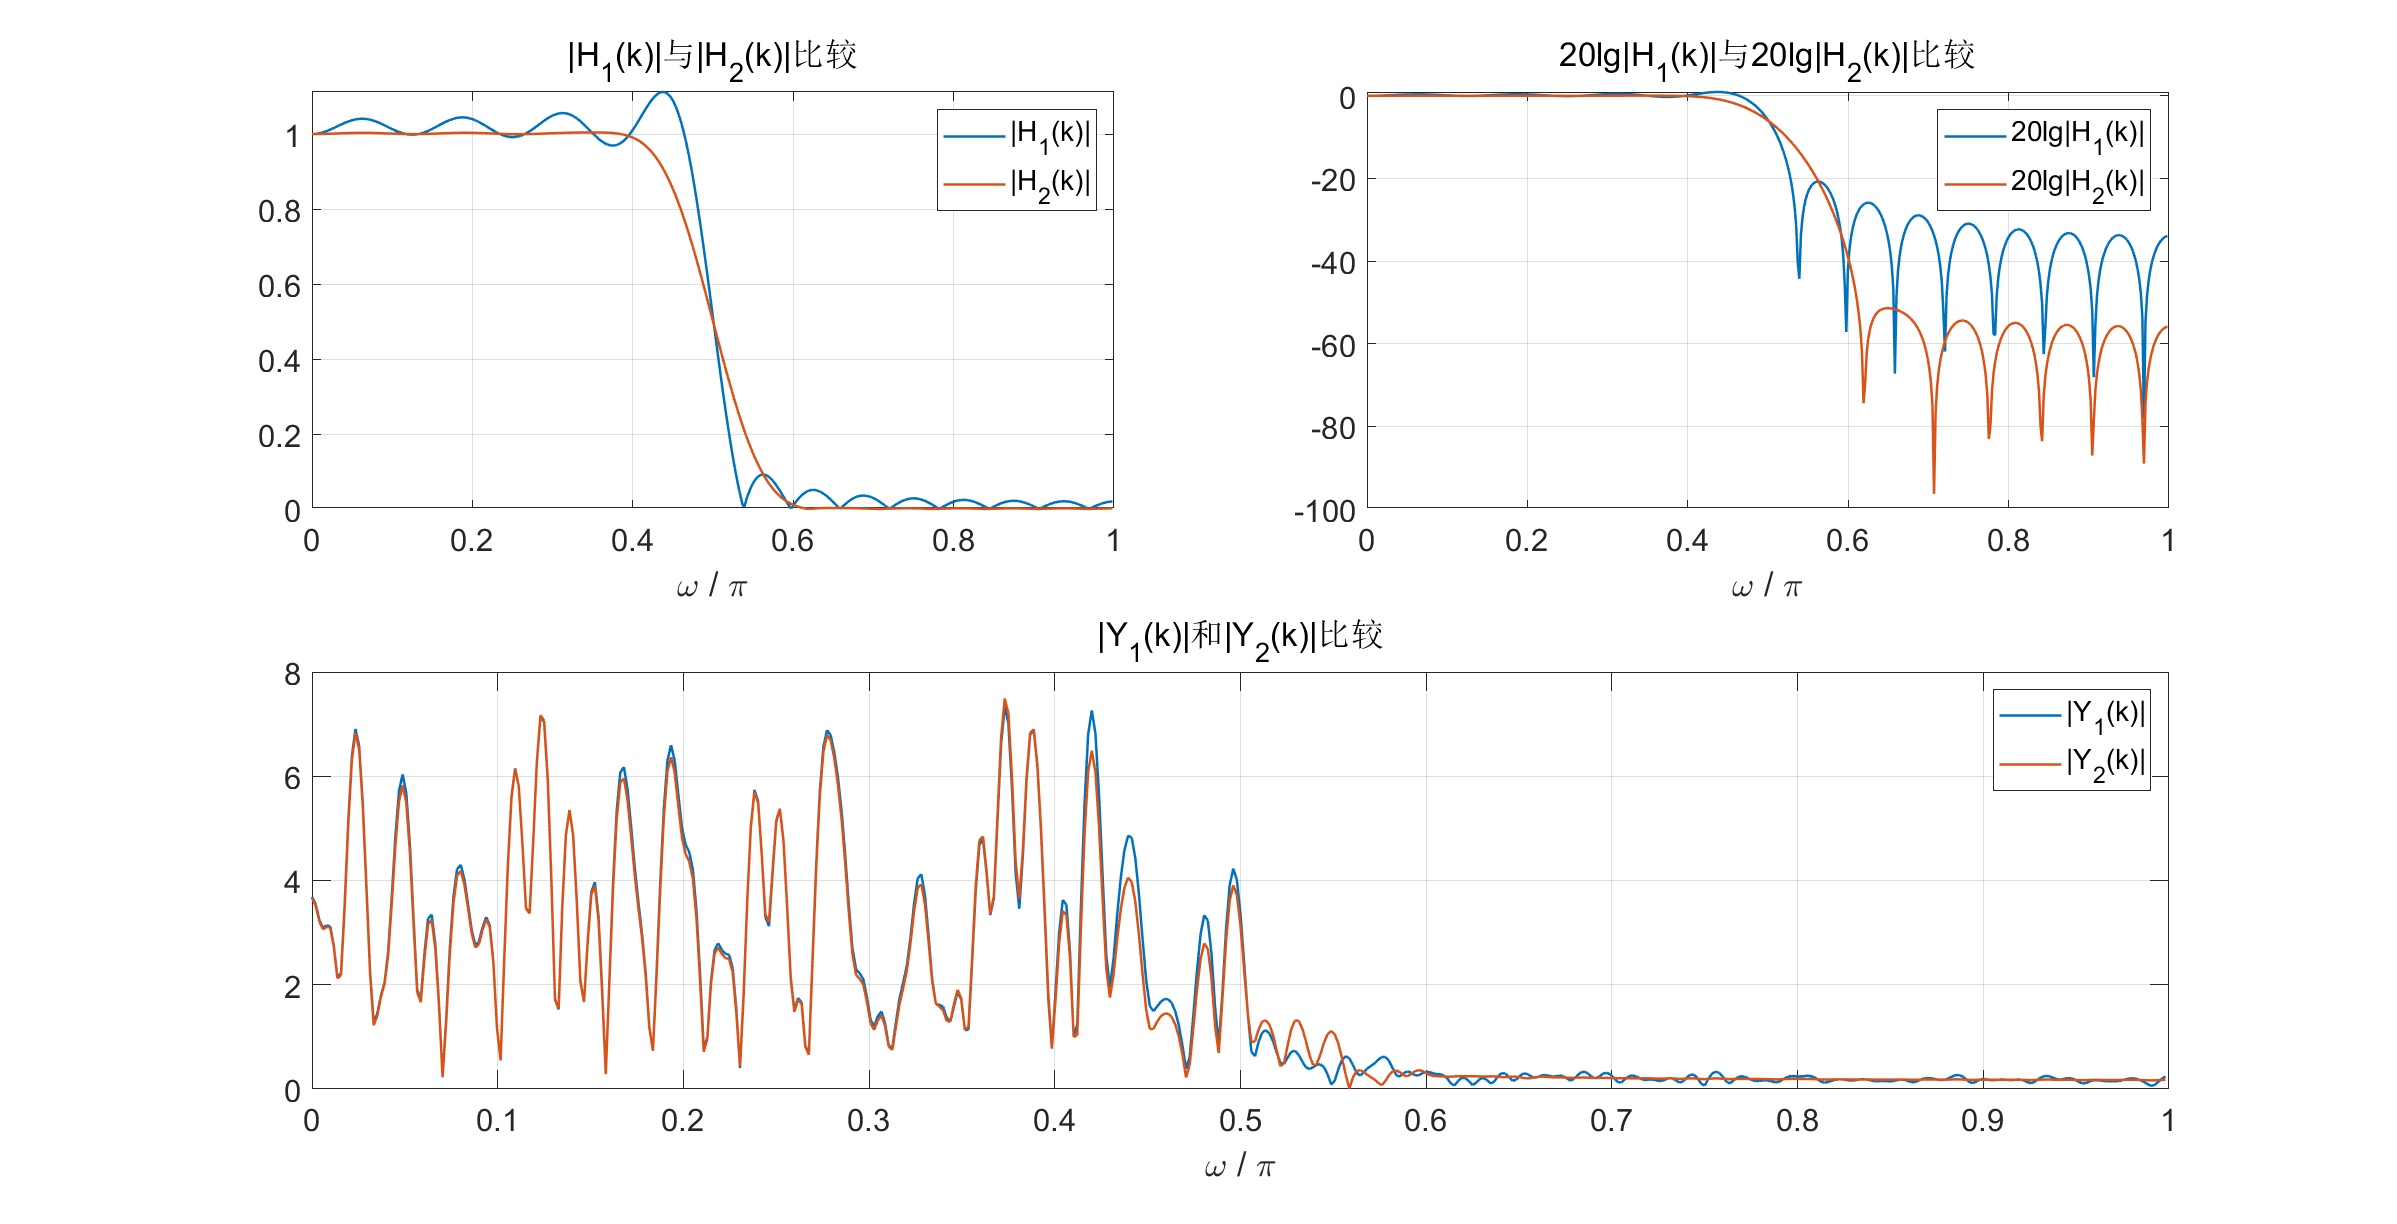
\includegraphics[width = 1\textwidth]{src/exp4-2-3-2.png}
\end{figure}
从图中可以看出,矩形窗和汉明窗设计的低通滤波器都做到了滤掉大部分的高频分量,基本保留低频分量。但是汉明窗设计的低通滤波器对高频分量的滤除更加好,但是在刚刚大于截至频率$\rm \omega _c = 0.5 \pi$之后,汉明窗设计的低通滤波器的输出信号衰减没有矩形窗好。

\subsection{2-4}
讨论不同的窗长设计出的滤波器的滤波效果。
\begin{figure}[H]
    \centering
    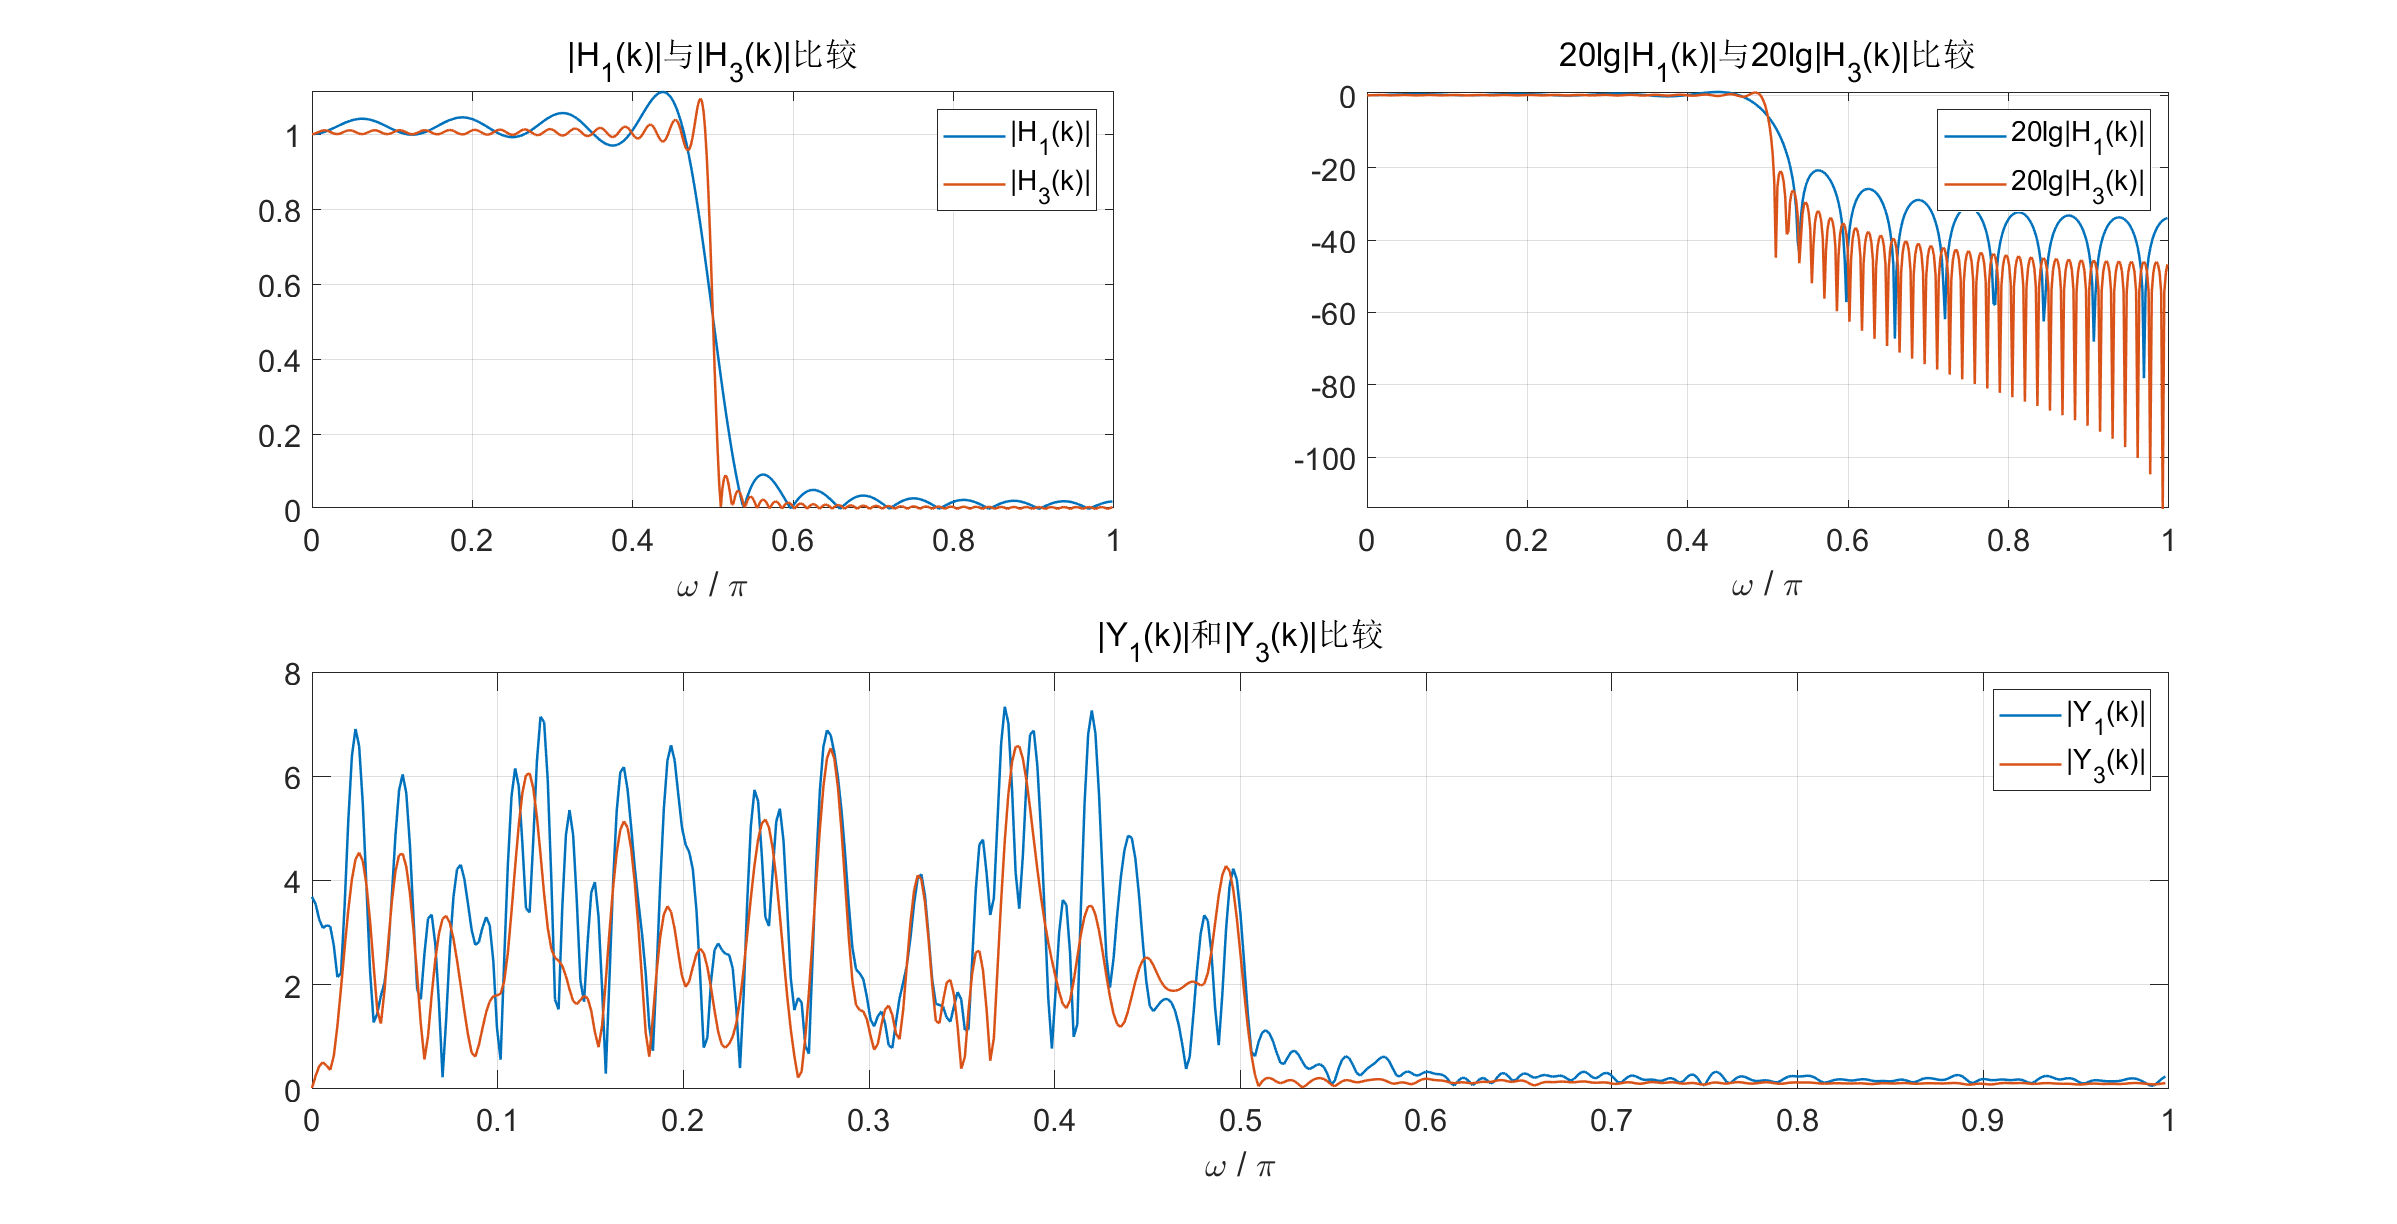
\includegraphics[width = 1\textwidth]{src/exp4-2-4.png}
\end{figure}
从图中可以看出,窗长为127的低通滤波器相对振荡幅度几乎不变,但是通带内波动更密集,过渡带变窄变抖。但两者的阻带最小衰减几乎相同。

总结:

从实验可以得出,滤波器的过渡带宽度由窗函数类型与窗长决定,其中矩形窗的过渡带更窄;窗函数相同时,窗长越长,过渡带越窄。

阻带最小衰减由窗函数类型决定,其中汉明窗的阻带衰减更大;而与窗长无关。

矩形窗设计的滤波器在阻带和通带内都存在波动,其中窗长更长的矩形窗设计出的低通滤波器通带内波动起伏更密,但相对振荡幅度却几乎不改变,证明了吉布斯效应的存在。而汉明窗设计的滤波器在阻带和通带内的波动非常小,几乎为0。

\end{document}